%%%%%%%%%%%%%%%%%%%%%%%%%%%%%%%%%%%%%%%%%%%%%%%%%%%%%%%%%%%%%%%%%%%%%%
% How to use writeLaTeX: 
%
% You edit the source code here on the left, and the preview on the
% right shows you the result within a few seconds.
%
% Bookmark this page and share the URL with your co-authors. They can
% edit at the same time!
%
% You can upload figures, bibliographies, custom classes and
% styles using the files menu.
%
%%%%%%%%%%%%%%%%%%%%%%%%%%%%%%%%%%%%%%%%%%%%%%%%%%%%%%%%%%%%%%%%%%%%%%

\documentclass[12pt]{article}

\usepackage{sbc-template}

\usepackage{graphicx,url}

\usepackage[brazil]{babel}   
\usepackage[utf8]{inputenc}  

     
\sloppy

\title{Explorando as Capacidades da Arquitetura UDP no\\ Desenvolvimento de Jogos Multiplayer para Android}

\author{João Walter Amadeu\inst{1}, Wesley Fantineli Bronzato\inst{1}, Rodrigo Moura Juvenil Ayres\inst{1} }


\address{BSI (Bacharelado em Sistemas de Informação) -
Rodovia BR 153, Km 338+420m, \\
Bairro Água do Cateto, Ourinhos-SP. CEP 19909-100
\email{\{joao.amadeu, 264033, rodrigo.ayres\}@unifio.edu.br}
}


\begin{document} 

\maketitle

\begin{abstract}
  The objective of this paper is to present the User Datagram Protocol (UDP) architecture and its main characteristics, through a real world use case - to develop a multiplayer game for Android using Kotlin, with the implementation of an UDP server also in Kotlin, and with the knowledge gathered through it, develop a methodology to compare the UDP architecture to TCP. Fundamental concepts of UDP architecture will be addressed, as well as its advantages and limitations. The goal of the developed game is to demonstrate the possibilities and benefits of using UDP in applications that require low latency and high performance.
\end{abstract}
     
\begin{resumo} 
  
O objetivo deste trabalho é apresentar a arquitetura User
Datagram Protocol (UDP) e suas principais características, e atráves de um caso de uso prático - desenvolver um jogo multiplayer para Android utilizando Kotlin, com a implementação de um servidor UDP também em Kotlin, e com o conhecimento obtido implementar uma metodologia para comparar a arquitetura UDP com TCP. Serão abordados conceitos fundamentais da arquitetura UDP, bem como suas vantagens e limitações. O jogo a ser desenvolvido terá como objetivo demonstrar as possibilidades e benefícios do uso de UDP em aplicações que exigem baixa latência e alta performance.
\end{resumo}


\section{Introdução}
A tecnologia de redes de computadores tem evoluído significativamente nas últimas décadas, e com ela, surgiram inúmeras oportunidades para o desenvolvimento de serviços em tempo real. A transmissão de dados em tempo real é uma necessidade comum em diversos tipos de aplicações, como jogos online, comunicação em tempo real, streaming de vídeo e muito mais.

Uma das tecnologias que permitem a transmissão de dados em tempo real é o User Datagram Protocol (UDP), que é um protocolo de transporte da camada de transporte do modelo OSI. O UDP oferece um mecanismo eficiente e rápido para transmitir dados pela rede, sem as restrições e sobrecargas adicionais do Transmission Control Protocol (TCP). Isso torna o UDP uma opção atraente para aplicativos que precisam de baixa latência e tempo de resposta rápido, como jogos em tempo real.

Neste trabalho, exploramos a tecnologia UDP, desenvolvendo um aplicativo de jogo da velha em tempo real que permite que os usuários criem salas e joguem o jogo com outros jogadores conectados ao servidor. O aplicativo foi desenvolvido em Kotlin para Android, e o servidor em Kotlin, implementando as funcionalidades necessárias para gerenciar as conexões entre os jogadores, transmitir as mensagens de jogo e garantir a integridade dos dados transmitidos.

Por fim, os protocolos TCP e UDP são comparados utilizando o conhecimento obtido durante o desenvolvimento do projeto de aplicativo, a fim de demonstrar efetivamente as vantagens do protocolo UDP para comunicação em tempo real.

\section{Fundamentação Teórica} \label{sec:firstpage}

A arquitetura de rede User Datagram Protocol (UDP) é uma tecnologia utilizada para a transferência de dados em redes de computadores. Diferente do Transmission Control Protocol (TCP), que é baseado em conexões e garante a entrega ordenada e confiável dos dados, o UDP é uma tecnologia que não garante a entrega dos dados, nem a sua ordem. Como afirma \cite{kurose2013computer}: "O UDP é um protocolo datagrama não confiável e sem conexão".

\subsection{TCP/IP}
O protocolo TCP/IP é um conjunto de protocolos de comunicação de rede que são usados para conectar computadores em redes. Ele foi desenvolvido na década de 1970 como parte do projeto ARPANET do Departamento de Defesa dos Estados Unidos. Segundo \cite{forouzan2018comunicacao}, o TCP/IP é amplamente utilizado na Internet e em muitas outras redes, incluindo redes locais e de longa distância. Ele é composto por dois protocolos principais: o Transmission Control Protocol(TCP) e o Internet Protocol (IP), que trabalham juntos para garantir a transferência confiável de dados na rede.

\cite{neuman2003redes} afirma que "O conjunto de protocolos TCP/IP é a fundação sobre a qual a Internet é construída. Ele é um conjunto de protocolos de comunicação que permite que computadores em redes diferentes possam se comunicar e trocar informações de forma confiável e eficiente".

De acordo com \cite{tanenbaum2011redes} o TCP/IP é composto por dois protocolos principais: o protocolo de controle de transmissão (TCP) e o protocolo de Internet (IP). O TCP é responsável pelo estabelecimento e manutenção de conexões confiáveis entre aplicativos em diferentes computadores, enquanto o IP é responsável pelo roteamento de pacotes de dados através de diferentes redes.

Segundo \cite{forouzan2018comunicacao} o protocolo TCP/IP é um protocolo de camada de rede. A camada de rede é responsável por fornecer uma rota de comunicação entre dois dispositivos em uma rede. O protocolo TCP/IP é a base da Internet, que é uma rede global de computadores. Ele permite que computadores de diferentes fabricantes e sistemas operacionais possam se comunicar e trocar informações.

Segundo \cite{tanenbaum2011redes} o protocolo TCP/IP é amplamente utilizado em muitas aplicações de rede, incluindo navegação na web, correio eletrônico, transferência de arquivos e compartilhamento de recursos.

De acordo com \cite{forouzan2018comunicacao}, o TCP/IP é um protocolo extremamente importante para a comunicação de rede. Ele é a base da Internet e é amplamente utilizado em muitas outras redes. Seu uso garante a comunicação confiável e eficiente de informações entre diferentes dispositivos em uma rede. O conhecimento do protocolo TCP/IP é fundamental para profissionais de rede e de tecnologia da informação que desejam trabalhar com redes de computadores.

\subsection{UDP}
De acordo com \cite{kurose2013computer}, a comunicação UDP é "um protocolo sem conexão que é simples e eficiente, mas não oferece garantias de que os pacotes de dados enviados serão entregues corretamente". Em outras palavras, a comunicação UDP é uma maneira simples e rápida de enviar dados entre dispositivos na rede, sem a sobrecarga de estabelecer uma conexão completa. No entanto, a falta de conexão também significa que a comunicação UDP não é tão confiável quanto o TCP, e alguns dados podem ser perdidos ou corrompidos durante a transmissão.

\cite{forouzan2018comunicacao} diz que "o UDP é um protocolo simples, sem conexão, que é usado principalmente para aplicativos que exigem uma transferência rápida de dados e que podem suportar algumas perdas de dados, como streaming de vídeo e jogos online". Ao contrário do TCP, que é orientado a conexão, o UDP não estabelece uma conexão antes de iniciar a transmissão de dados. Isso significa que os pacotes de dados podem ser enviados sem nenhuma confirmação ou controle de erro. Isso torna a comunicação UDP menos confiável do que o TCP, mas também mais rápida e eficiente em redes com alta latência ou com um grande número de pacotes pequenos.

Um recurso interessante da comunicação UDP é o seu suporte a broadcast e multicast. Com o UDP, é possível enviar um pacote de dados para vários dispositivos ao mesmo tempo, sem a necessidade de retransmitir o pacote para cada destinatário individualmente. Isso é especialmente útil em aplicações como videoconferência, onde vários participantes precisam receber os mesmos dados simultaneamente. De acordo com \cite{tanenbaum2011redes}, O UDP é o protocolo ideal para enviar datagramas para múltiplos destinatários, porque os datagramas podem ser enviados uma única vez e chegar a múltiplos receptores".

Uma das desvantagens da comunicação UDP é a falta de mecanismos de controle de congestionamento. Diferente do TCP, que faz uso de um algoritmo de controle de congestionamento para ajustar a taxa de transmissão de dados em função do tráfego da rede, o UDP não possui mecanismos de controle de congestionamento. Isso significa que, se a taxa de transmissão de dados for maior do que a capacidade da rede, os pacotes de dados podem ser perdidos ou descartados, comprometendo a qualidade da transmissão. De acordo com \cite{stallings2017redes}, "sem controle de congestionamento, o UDP é incapaz de regular o fluxo de tráfego e não pode detectar quando a rede está congestionada. Em vez disso, os datagramas UDP são enviados para a rede na taxa máxima possível e a rede deve lidar com eles da melhor maneira possível"


Em resumo, a comunicação UDP é um protocolo de transporte sem conexão que oferece uma transmissão de dados rápida e eficiente, mas menos confiável do que o TCP. De acordo com \cite{tanenbaum2011redes}, Sua natureza sem conexão e suporte a broadcast e multicast o torna uma opção atraente para aplicações que exigem alta performance, como jogos online e streaming de vídeo. No entanto, sua falta de mecanismos de controle de congestionamento torna a comunicação UDP menos adequada para aplicações que exigem alta confiabilidade, como transações financeiras online.

\subsection{Kotlin}
A linguagem Kotlin é uma linguagem de programação moderna, de código aberto, que roda na máquina virtual Java (JVM) e também pode ser compilada para JavaScript. Segundo \cite{subramaniam2017programming}, "Kotlin é uma linguagem que tenta equilibrar a concisão da sintaxe com a legibilidade do código, a facilidade de aprendizado com o poder de expressividade, e a interoperabilidade com a simplicidade."

Dentre as principais vantagens da linguagem Kotlin em relação ao Java, destaca-se a sintaxe mais limpa e expressiva. De acordo com \cite{jemerov2017kotlin}, "o Kotlin tem uma sintaxe mais concisa do que o Java, o que significa que você precisa digitar menos código para realizar as mesmas tarefas." Essa característica torna o Kotlin mais fácil de ler, escrever e manter.

Outra vantagem importante do Kotlin é o Null Safety. Segundo \cite{leiva2019kotlin} "Null safety significa que você não precisa se preocupar com exceções de ponteiro nulo." Em outras palavras, é possível garantir que um objeto nunca seja nulo, o que ajuda a evitar erros comuns de programação.

Além disso, o Kotlin oferece recursos interessantes, como inferência de tipos, lambdas e funções de extensão.\cite{mccarthy2019kotlin} diz que "a inferência de tipos é uma das características mais fortes do Kotlin", pois "permite que o compilador descubra o tipo de uma variável sem que o programador precise especificá-lo". Já as lambdas e funções de extensão tornam o código mais conciso e expressivo.

Por fim, vale destacar que o Kotlin tem ganhado popularidade como uma alternativa ao Java para desenvolvimento de aplicativos Android. Segundo \cite{leiva2019kotlin} "o Kotlin é uma linguagem muito adequada para o desenvolvimento de aplicativos Android, devido à sua interoperabilidade com o Java e à sua compatibilidade com a JVM." Isso significa que é possível utilizar o Kotlin em conjunto com o Java, o que facilita a transição e a manutenção de código legado.

\subsection{Android}
\cite{gazzola2020desenvolvimento} diz que o sistema operacional Android é uma plataforma móvel baseada em Linux desenvolvida pelo Google e utilizada em diversos dispositivos móveis, como smartphones, tablets, smartwatches e televisões. O Android é uma plataforma de código aberto e permite que desenvolvedores criem aplicativos para o sistema utilizando as linguagens de programação Java ou Kotlin.

Para desenvolver aplicativos para Android, de acordo com \cite{sarkar2020android}, é necessário utilizar uma ferramenta de desenvolvimento integrado (IDE) chamada Android Studio. O Android Studio é uma IDE gratuita e oficial do Google, que fornece uma variedade de recursos para auxiliar os desenvolvedores na criação de aplicativos para Android, como um editor de código, um depurador, um emulador de dispositivo, entre outros.

De acordo com \cite{gazzola2020desenvolvimento} Uma das principais características do Android é o seu modelo de permissões de segurança, que define o acesso que um aplicativo tem aos recursos do dispositivo. Cada aplicativo é executado em sua própria sandbox, o que significa que ele não pode acessar os recursos de outros aplicativos sem permissão explícita do usuário. Além disso, o Android utiliza recursos de segurança adicionais, como a verificação de integridade de aplicativos e a criptografia de dados em repouso.

Por fim, de acordo com \cite{sarkar2020android} o desenvolvimento de aplicativos para Android também envolve a criação de interfaces de usuário (UI) eficazes e agradáveis para o usuário. O Android fornece uma variedade de recursos de UI, como layouts, widgets, estilos e temas, que podem ser utilizados para criar interfaces de usuário atraentes e funcionais.

\subsection{Trabalhos correlatos}

\subsubsection{Arquitetura cliente-servidor em jogos multiplayer}

\cite{picoli2011arquitetura} realizou uma análise de padrões de comunicação  User Datagram Protocol (Protocolo de Datagrama do Usuário - UDP) para jogos eletrônicos multijogadores, baseado na arquitetura cliente-servidor. Esse estudo resultou, de acordo com seu autor, em uma arquitetura de comunicação aprimorada, aumentando a eficiência do sistema desenvolvido no projeto.

\subsubsection{Aplicação de controle remoto usando jogos sérios baseado no protocolo de comunicação UDP}

\cite{moreno2019aplicaccao} fizeram estudo sobre a escalabilidade e possibilidade do uso de comunicações UDP com a finalidade de controlar robôs e transferir dados entre placas de desenvolvimento. Concluiu-se que o protocolo UDP permite uma transferência de dados altamente eficiente, de alta taxa de velocidade e altamente escalável.

\subsubsection{Desenvolvimento de aplicativo para adoção de animais abandonados utilizando a linguagem de programação Kotlin e programação reativa}
\cite{silva2017desenvolvimento} desenvolveu uma aplicação que permite a adoção de animais abandonados, e avaliou a linguagem Kotlin como a melhor para desenvolvimento de aplicações Android nativamente, contando com todos os conceitos mais modernos para apps da plataforma. Além disso, o autor também ressalta que a linguagem é a favorita pelo Google, principal mantenedor do Android, para desenvolvimento para a plataforma.

\section{Ferramentas e Tecnologias}
\label{sec:ferramentastecnologias}
Este capítulo apresenta as tecnologias Kotlin e UDP, e as ferramentas Android Studio e IntelliJ IDEA, que foram utilizadas no desenvolvimento do sistema proposto. A escolha dessas tecnologias e ferramentas foi motivada pela necessidade de uma linguagem moderna e eficiente, bem como de protocolos de comunicação robustos e confiáveis para a transmissão de dados entre dispositivos. Além disso, as ferramentas selecionadas oferecem um ambiente de desenvolvimento integrado (IDE) completo e poderoso para simplificar o processo de desenvolvimento e aumentar a produtividade.
\subsection{Kotlin}

\cite{leiva2019kotlin} diz que o Kotlin possui várias qualidades-chave que o tornam uma linguagem de programação valiosa para o desenvolvimento de software moderno. Em primeiro lugar, é altamente expressivo, permitindo uma codificação mais eficiente com menos linhas de código. Além disso, o Kotlin tem null safety, o que significa que situações potenciais onde valores seriam nulos são tratadas durante a compilação, reduzindo a ocorrência de exceções de tempo de execução e economizando tempo depurando problemas de ponteiro nulo. A linguagem também apresenta muitos conceitos da programação funcional, incluindo expressões lambda, para solução de problemas mais fácil, e oferece tratamento de coleções simplificado. Além disso, o Kotlin faz uso de funções de extensão, que permitem a extensão de qualquer classe com novos recursos, mesmo sem acesso ao código-fonte. Por fim, a interoperabilidade do Kotlin com o Java é excelente, permitindo que os desenvolvedores continuem usando a maioria das bibliotecas e código escrito em Java e até mesmo criando projetos mistos que utilizam arquivos em Kotlin e Java.


De acordo com \cite{jemerov2017kotlin}, o Kotlin funciona muito bem com todas as bibliotecas e frameworks Java existentes e roda com o mesmo nível de desempenho que o Java. As características da linguagem Kotlin, combinadas com um plug-in especial do compilador que suporta o framework Android, transformam o desenvolvimento Android em uma experiência muito mais produtiva e agradável. Tarefas de desenvolvimento comuns, como adicionar ouvintes aos controles ou vincular elementos de layout a campos, podem ser realizadas com muito menos código, ou às vezes sem código algum (o compilador gerará o código para você).

\subsection{UDP}
\cite{stevens2011tcp} diz que o Protocolo de Datagrama de Usuário (UDP) é um protocolo de camada de transporte simples e orientado a datagramas que preserva as fronteiras das mensagens. Diferentemente do TCP, UDP não oferece correção de erros, sequenciamento, eliminação de duplicatas, controle de fluxo ou controle de congestionamento. No entanto, o protocolo fornece detecção de erros e inclui o primeiro checksum verdadeiramente end-to-end da camada de transporte. Por não oferecer funcionalidades mais complexas, o UDP permite que as aplicações que o utilizam tenham controle total sobre como os pacotes são enviados e processados. No entanto, isso significa que as aplicações precisam implementar seus próprios mecanismos de proteção para garantir a entrega confiável e sequenciada dos dados.

\subsection{Intellij IDEA}
\cite{saunders_fields_belayev_2013} diz que o IntelliJ IDEA é uma plataforma de desenvolvimento integrado (IDE) de última geração para a linguagem de programação Java. Como o termo IDE sugere, o IDEA reúne todas as ferramentas necessárias para o desenvolvimento de software Java em uma única aplicação e interface. Em resumo, o IDEA é uma ferramenta que auxilia no desenvolvimento de aplicativos Java de forma mais rápida, fácil e inteligente. Ele pode ser usado em todas as fases do projeto, desde o planejamento e desenvolvimento até os testes e implantação.


\subsection{Android Studio}
De acordo com\cite{smyth2020android}, O desenvolvimento de aplicativos para o Android envolve uma quantidade considerável de trabalho de programação, que, por definição, envolve digitar, revisar e modificar linhas de código. Não é surpresa que a maioria do tempo de um desenvolvedor usando o Android Studio seja gasto editando código na janela do editor. O editor de código moderno precisa ir muito além dos princípios básicos de digitar, excluir, cortar e colar. Hoje, a utilidade de um editor de código é geralmente avaliada por fatores como a quantidade pela qual reduz a digitação necessária pelo programador, a facilidade de navegação por grandes arquivos de código-fonte e a capacidade do editor de detectar e destacar erros de programação em tempo real, enquanto o código está sendo escrito. Como ficará evidente neste capítulo, esses são apenas alguns dos aspectos em que o editor do Android Studio se destaca. Embora não seja uma visão geral exaustiva dos recursos do editor do Android Studio. Programadores experientes descobrirão que alguns desses recursos são comuns à maioria dos editores de código disponíveis hoje, enquanto outros são exclusivos deste ambiente de edição particular.

Com base nessas características, foi feita a instalação do JDK, IntelliJ IDEA e Android Studio no computador. Em seguida, criamos um novo projeto Kotlin no IntelliJ IDEA, que serve como servidor para nossa aplicação Android, o cliente. Criamos também o projeto do aplicativo Android no Android Studio

\section{Desenvolvimento}
O trabalho presente tem como objetivo demonstrar a tecnologia UDP por meio do desenvolvimento de um aplicativo de jogo da velha em tempo real. Isso permite que os usuários criem salas e joguem o jogo com outros jogadores conectados ao servidor. Para alcançar esse objetivo, desenvolvemos um aplicativo para Android e um servidor, ambos utilizando a linguagem Kotlin.

O primeiro passo do processo de desenvolvimento foi a definição dos requisitos do projeto. Foi fundamental determinar as funcionalidades que o aplicativo deveria ter para atender aos objetivos do projeto, como a criação de salas, a conexão entre clientes, a transmissão de mensagens em tempo real e a jogabilidade do jogo da velha.

Para o desenvolvimento do aplicativo, escolhemos o Android Studio e a linguagem Kotlin. Para o servidor, optamos pela biblioteca Ktor e Kotlin. Além disso, para implementar o protocolo UDP, utilizamos a API DatagramSocket.

O próximo passo foi o desenvolvimento do servidor em Kotlin, que recebe as conexões dos clientes e gerencia as salas de jogo. Implementamos as funcionalidades de criação de salas, conexão e desconexão de clientes, além de garantir que as mensagens fossem enviadas de forma segura e em tempo real usando o protocolo UDP.

O desenvolvimento do aplicativo foi a etapa seguinte, permitindo que os usuários se conectem ao servidor e joguem o jogo da velha em tempo real. O aplicativo foi projetado para ser intuitivo e fácil de usar, permitindo que os usuários criem e se juntem a salas de jogo, e joguem o jogo da velha de forma fluida e eficiente.

Após o desenvolvimento do aplicativo e do servidor, realizamos testes e depuração do sistema para garantir que estivesse funcionando corretamente. Testamos todas as funcionalidades, incluindo a conexão com o servidor e a jogabilidade do jogo da velha.

Além disso, desenvolvemos outro conjunto de aplicações com o intuito de comparar sinteticamente os protocolos UDP e TCP.

Com os testes e depuração concluídos, implementamos as funcionalidades finais do aplicativo e do servidor, incluindo melhorias na interface do usuário e o aprimoramento do desempenho.

O código fonte do projeto está disponível no GitHub em  https://github.com/fortmea/apptcc para o aplicativo e https://github.com/fortmea/servidortcc para o servidor.

\section{Resultados}

\begin{figure}[ht]
\centering
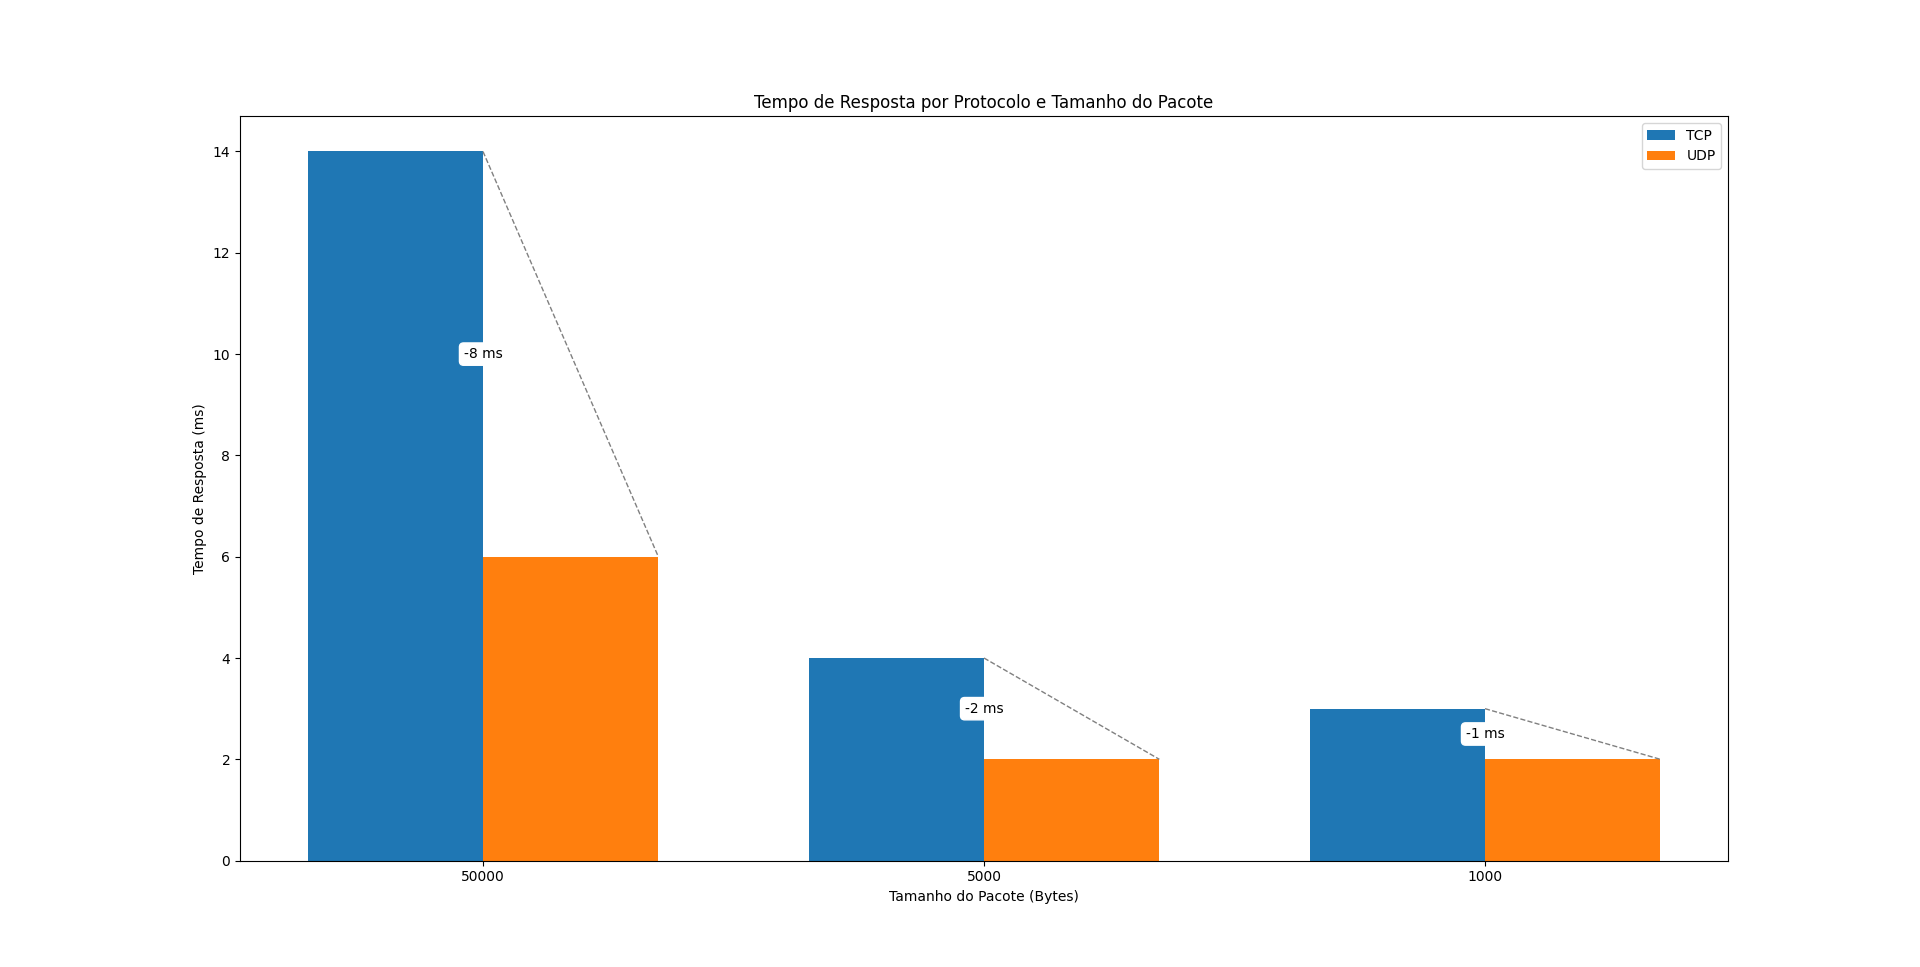
\includegraphics[width=1\textwidth]{grafico_ms.png}
\caption{Tempo de Resposta por Protocolo e Tamanho do Pacote}
\label{fig:cronogramafig}
\end{figure}

\bibliographystyle{sbc}
\bibliography{sbc-template}

\end{document}
